%Contributer: Kendal Sandridge, Colin Tan
{\parindent0pt
\section{Spectral Clustering}

As of late Spectral Clustering has become exceedingly popular due to the quality of its clusters compared to other clustering algorithms.   It is possible to turn clustering into a graph problem, then solve it by figuring out the cut that splits our graph into the groups with high intracluster weights. One of the benefits of this formulation is that the data can be in any space, not just euclidean, and we can still perform clustering. \\

We can formulate the problem of spectral clustering with well defined inputs and outputs

\textbf{Input:} \\
- $x_1,...,x_n$ data points\\
- $w_{ij}$ similarity between points $x_i, x_j$ \\

\textbf{Goal}\\
- MINIMIZE intercluster weights\\
- MAXIMIZE intracluster weights\\



We first introduce the notion of a similarity graph. We can construct a similarity graph from a set of points $S$, and a similarity function that returns a value $s_{ij}$, the similarity from points $i, j \in S$. In this way we construct a graph $G = (V,E)$ where $V = S$ and $(i,j) \in E$ if $s_{ij} > 0$.  The weights of each edge in the weights matrix would be $s_{ij}$ if $s_{ij}$ is positive and 0 otherwise. There are actually many ways of constructing the weight matrix $W$ of $G$. A few are listed below:\\

\textbf{Methods of creating W}
\begin{itemize}
	\item k-NN graph
	\item $\epsilon$-neighbor graph
	\item Gaussian kernel $w_{ij} = exp(\dfrac{-\lVert x_i - x_j\rVert ^2}{2 \sigma ^2})$
\end{itemize}

A few facts about the weights matrix is that if $w{ij} = 1 \Longleftrightarrow (i,j) \in E$, then $W$ is the usual adjacency matrix. Also $W$ is symmetric. \\


We can define the degree of the a vertex, $v \in V$ to be:
\begin{center}
	\[ d_i := \sum_{j \in V} w_{ij}\]
\end{center}

From this we can also define a degree matrix, $D$:
\begin{center}
	$D = diag(d_i, ..., d_n)$	
\end{center}

\textbf{Useful Notation}\\
It is also helpful to define an edge function $E(S,T)$:
\begin{center}
	Given that $S, T \subset V$ $ E(S,T) := \{(i,j) \in E : i \in S, j \in T\}$\\
\end{center}

We denote the compliment of a set of vertices, $\bar{S}$ as:
\begin{center}
	$\bar{S} := S \setminus V$
\end{center}

For shorthand we denote:
\begin{center}
	$\delta S = E(S, \bar{S})$
\end{center}

It is also important to have a notion of size for a set of vertices. The first is simply the cardinality of the set. The second is the volume of the set defined below.
\textbf{Measures of Size} $S \subset V$: \\
\begin{center}
	\item \[vol(S) := \sum_{i \in S} d_i = \sum_{\substack{i\in S \\
			j\in V}} w_{ij} = weight(E(S, V))\]
\end{center}


\textbf{The MINCUT Problem}\\
\[  \underset{{\emptyset \varsubsetneq S \varsubsetneq V}}{\mathrm{min}}  weight(E(S,\bar{S})) = weight(\delta S) \]\\

\textbf{Fact} \textit{(Stoer-Wagner, 1995)}. There is an efficient algorithm that solves MINCUT.\\
	
	Question: Is this good for clustering?\\
	A: No. We can try to "balance" the size of each partition but turns out the problem become NP-hard \textit{(Wagner \& Wagner 19)}\\
	
	\subsection{Spectral Graph Theory}
	At its heart, the graph Laplacian, L.
	
	\textbf{Review of Laplacian}
	$G = (V,E)$
	Dictionary between discrete calculus \& vector calculus:

	\begin{multicols}{2}
		\textbf{Discrete Calculus}\\
		\begin{itemize}
		\item $V$ is sparse  
		\item $\mathbb R^V$ is space of vertex functions\\
			 inner product space: $\langle f,g\rangle_v := \sum_{i\in V} f(i)g(i)$
		
		\item $\mathbb R^E$ is space of alternating vertex functions
			 \[X([i,j] = -X([j,i]) \textrm{for} (i,j) \in E \]
			inner product space: \[\langle X,Y\rangle_E := \sum_{e \in E} w_e X(e) Y(e) \]
		\item $d$ the derivative operator
		\[d: \mathbb R^V \rightarrow \mathbb R^E\]
		\[ df([i,j]) = f(j)-f(i)\]
		\item Dirichlet energy, measure of smoothness
		\[\mathcal E(f) := \langle df,df\rangle_E = \sum_{\substack{(i,j)\\
				{i < j}}} w_{ij} (f(i)-f(j))^2\]\\
		\end{itemize}
		\columnbreak
		\textbf{Vector Calculus}
		\begin{itemize}
			\item $\mathcal M$ is sparse
			\item $\mathcal C^{\infty}(\mathcal M; \mathbb R)$ space of functions 
			\item $\nabla$ gradient operator
			\item $\mathcal E(f) := \int_{\mathcal M} \lVert \nabla f \rVert ^2$
		\end{itemize}
	\end{multicols}
	Recall the adjoint.\\
	\begin{center}
		if $T: A \rightarrow B$ map of finite-dimension inner product spaces, then\\
		$\exists! T*: B \rightarrow A$ s.t. $\forall a \in A, b \in B, <a, Ta>_B = \langle T*b, a\rangle_A$
	\end{center}
	
	The Laplacian $L$ defined so that:
	\begin{center}
		$\langle df, df\rangle_E = \langle f,Lf\rangle_V$
	\end{center}
	
	Why consider L? In order to form an optimization problem!
	e.g. 
	\begin{center}
		$min \langle df, df\rangle_E $ \indent Lagrange Multipliers $\rightarrow Lf = \lambda f$\\
		s.t. \[ \lVert f \rVert ^2 = 1 \]
	\end{center}
	
	\textbf{Properties of Laplacian}
	\begin{enumerate}
		\item $L = D - W$
		\item $\mathbbm{1} \in ker(L)$
		\item $L \in Sym(\mathbbm R^{n\times n})$
		\item let $A \subset V$. $\mathbbm 1_A^T L \mathbbm 1_A = \sum_{(i,j) \in E} w_{ij} (\mathbbm  1_A(i - \mathbbm 1_A(j)) )^2 = weight(E(A, \bar{A})) $
	\end{enumerate}
	
	\subsection{Review of Spectral Theory: Geometric \& Variational Characterization of Eigenvalues}
	
	\begin{definition}
		Let $M \in \mathbb R^{n \times n}$. An eigenvector $v \in \mathbb R^n$ satisfies $v \neq 0, \exists\lambda \in \mathbb R $ s.t. $Mv = \lambda v$
		The eigenvalues of this matrix form its spectrum.
	\end{definition}
	
	\begin{theorem}[Spectral Theorem for Symmetric Matrices]
		
		Geometric characterization
		
		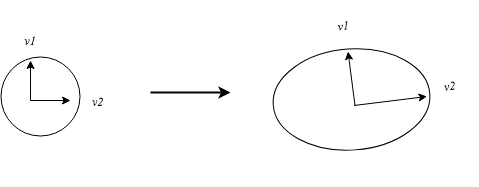
\includegraphics[width=0.8\textwidth]{chapter_3/files/spec_clust_diag.png}
	\end{theorem}
	
	\begin{definition}
		Let $v \neq 0 $ in $\mathbb R^n, \mathcal M \in Sym(\mathbb R{n \times n})$
		Rayleigh Quotient
		$\mathcal R(v) = \dfrac{v^T M v}{v^Tv}$
		
		Notice: $\mathcal R(\alpha v) = Rank(v) \forall \alpha \in \mathbb R \ \{0\}$, can assume $v \in S^{n-1}$
	\end{definition}
	
	
	\begin{theorem}[Variational Characterization]
		Let $M \in Sym(\mathbb R^{n\times n})$\\
		$\lambda_1 \leq ... \leq \lambda_n$ eigenvalues of $M$ \\
		$\lambda_1 = \min_{v \in S^{n-1}} Rank (v)$\\
		$\vdots$ \\
		$\lambda_i = \min_{\substack{ v \in S^{n-1}\\
				v \perp < v_1 ... v_{i-1} >}} Rank (v)$ \\
		$\vdots$ \\
		$\lambda_m = \max_{v \in S^{n-1}} Rank (v)$
	\end{theorem}
	
	\subsection{Spectral Clustering Algorithm}
	
	The algorithm needs predefined number of clusters, and the similarity matrix.
	
	\textbf{Input:} $S$: $n\times n$ similarity matrix (on $n$ datapoints), $k$: number of clusters.
	
	\textbf{Output:} the partition of $n$ datapoints returned by $k$-means as the clustering.
	
	\begin{enumerate}
		\item Compute the degree matrix $D$ and adjacency matrix $W$ from the weighted graph induced by $S$.
		\item Compute the graph Laplacian $L = D - W$.
		\item Compute the bottom $k$ eigenvectors $u_1,\ldots,u_k$ of the generalized eigensystem $\mathbf{Lu} = \lambda \mathbf{Du}$.
		\item Let $U$ be the $n \times k$ matrix containing vectors $u_1,\ldots,u_k$ as columns.
		\item Let $y_i$ be the $i$-th row of $U$; it corresponds to the $k$ dimensional representation of the datapoint $x_i$.
		\item Cluster points $y_1,\ldots,y_n$ into $k$ clusters via a centroid-based algorithm like $k$-means.
	\end{enumerate}
	
	One can calculate similarity from distance using a drop off function $e^{-\mathrm{dist}^2/\sigma^2}$.
	
	\subsection{Planted Partitions Model}
	
	The need to calculate the eigenvector of the $n\times n$ Laplacian puts the spectral clustering algorithm at $O(n^3)$ runtime. There is an $O(n \log^3 n + m \log n)$ algorithm for Planted Partitions Model problem, as described in \cite{bsh10}.
	
	The Planted Partitions Model problem: for a $(p,q)$-clusetered graph $G(V,E)$, vertices are divided into disjoint clusters $C_1, \ldots, C_t$. Edges between members within clusters are included with probability $p$, and between members across clusters with probability $q$.
	
	Note that $C(v)$ is the cluster containing vertex $v$, and $N(G,v)$ are the neighbors of $v$.
	
	For $p \geq 1/2$, the following Subsquare algorithm described in \cite{bsh10} finds partitions $U_1, \ldots, U_s$ with probability $1-1/\mathrm{poly}(n)$ that for each input cluster $C_i$ of size $\Omega(\max \{qn, \log n \})$, contains a cluster $U_j$ such that $C_i=U_j$. The algorithm takes three parameters, $c_0$, $c_1$, and $\delta$.
	
	\begin{itemize}
		\item Randomly order the the vertices with a bijection $\pi : V \rightarrow \{1, \ldots, n\}$.
		\item Run two passes of the following for each $v$:
		\begin{enumerate}
			\item If $|N(G,v)|<c_0 \log(n/\delta)$, assign $v$ to its own cluster and continue to the next $v$.
			\item Let $R_{temp}$ be the neighbors of $v$ that have been clustered.
			\item For each element of $R_{temp}$, include it in $R$ with probability $\min \left\{\frac{c_{0} \log (n / \delta)}{\left|R_{t e m p}\right|}, 1\right\}$.
			\item For each element of $N(G,v)$, include it in $S$ with probability $\frac{c_{0} \log (n / \delta)}{|N(G, v)|}$. Similarly for each element of $N(G,w)$, include it in $S_w$ with probability $\frac{c_{0} \log (n / \delta)}{|N(G, w)|}$.
			\item Initialize a candidate cluster set $\mathcal{D}$ for $v$ to empty set.
			\item For each $w \in R$, if
				\begin{enumerate}
					\item $|S \cap N(G, w)| \geq c_{1} \log (n / \delta)$,
					\item $|N(G, w)| \geq c_{0} \log (n / \delta)$ and $\left|S_{w} \cap N(G, v)\right| \geq c_{1} \log (n / \delta)$,
				\end{enumerate}
				add $w$'s cluster $\hat{C}(w)$ to $\mathcal{D}$.
			\item If $\mathcal{D}$ is not empty, set $\hat{C}(v)=\hat{C}\left(\operatorname{argmin}_{w^{\prime} \in \cup_{C \in \mathcal{D}}} \pi\left(w^{\prime}\right)\right)$. Else, assign $v$ to its own cluster.
		\end{enumerate}
	\end{itemize}
	
	The correctness and runtime are bounded by the following theorems:
	
	\begin{theorem}
		There are constants $c, \delta_{0}, m_{0}$ and $n_{0}$ such that, for all $p \in[1 / 2,1], q \in[0,1], m \geq m_{0}$, $n \geq n_{0},$ and $0<\delta \leq \delta_{0},$ if $G$ is a $(p, q)$ clustered graph with clusters $C_{1}, \ldots, C_{t},$ then, with probability $1-\delta$, Algorithm Subsquare, when run with $c_{0}=c / 2$ and $c_{1}=c / 2^{5},$ outputs a partition $U_{1}, \ldots, U_{s}$ of the vertices of $G$ such that, for all cluster indices $i$ such that
			\begin{equation}\label{eq:bsh10-eq1}
				\left|C_{i}\right| \geq c \max \{q n, \log (n / \delta)\}
			\end{equation}
			there is a output cluster index $j$ such that $C_{i}=U_{j}$.
	\end{theorem}
	
	Define the edge test to be a check of the conditions in the algorithm step 6. If the conditions are satisfied, and $C(v)=C(w)$, or the conditions are not satisfied and $C(v) \neq C(w)$, then the edge test succeeds, otherwise it fails.
	
	\begin{lemma}
		With probability $1-\delta/\mathrm{poly}(n)$, for any vertex $v$ whose cluster $C(v)$ satisfies (\ref{eq:bsh10-eq1}), at least half of $v$’s neighbors are in $C(v)$.
	\end{lemma}
	
	\begin{lemma}
		For a pair $\{ v, w \}$ of vertices, if $C(v) = C(w)$, and the cluster satisfies (\ref{eq:bsh10-eq1}), and an edge test is conducted for $v$ and $w$, then, with probability $1-\delta/\mathrm{poly}(n)$, this edge test succeeds.
	\end{lemma}
	
	Which can be deduced using Chernoff bound from the test condition defined in algorithm step 6. Symmetrically,
	
	\begin{lemma}
		For any pair $\{ v, w \}$ of vertices, if $C(v)$ satisfies (\ref{eq:bsh10-eq1}), and an edge test is conducted between $v$ and $w$, and $C(v) \neq C(w)$, then with probability $1-\delta/\mathrm{poly}(n)$ the edge test is successful.
	\end{lemma}
	
	Then it proves that during the first pass, the first identified member (the head) of a cluster indeed forms a good cluster around it, i.e. for any vertex $v$ with an edge to the head $v_C$ of $C$, with probability $1-\delta/\mathrm{poly}(n)$, $C(v) = C(v_C)$. Reader can refer to the original paper for the full length of the proof.
	
	\begin{theorem}
		The expected running time of Subsquare is $O(n(\log ^{2}(n / \delta))(\log n)+m \log n)$.
	\end{theorem}
	
	Because the algorithm:
	
	\begin{itemize}
		\item Create a structure in $O(m \log n)$ time, like a balanced binary tree, to test neighborhood membership, i.e. if a vertex $w$ is in $N(G,v)$, in $O(\log n)$ time.
		\item For each vertex at most $O(\log(n/\delta))$ candidate clusters are examined, and each candidate requires neighbor lookups for $O(\log(n/\delta))$ neighbors.
	\end{itemize}
	
	
	
	\begin{exercise}
		let $M \in Sym(\mathcal R^{n \times n})$
		$min_{x} \sum_{i=1}^{n} x_i^T M x_i$ $min_(X) Tr(X^T M X)$ s.t. $X^TX = Id_{k\times k}$ 
		
		Q if $X$ minimizes this prob, is $X$ unique?\\
		A No. Let $U$ be an orthogonal matrix.  Consider $XU$. \\
		Claim: $XU$ is also optimal\\
		
		Fact $Tr(ABC) = Tr(BCA)$ \\
		
		\begin{center}
			$Tr(XU)^T M (XU)$\\
			$ Tr(X^T M X)$ given $(XU)^T(XU) = Id$
			$=Tr(X^TMX)$
		\end{center}
		
	\end{exercise}
}

